%{{{-----------------------------------Basics----------------------------------%

%document class definition
\documentclass[
    11pt,
    a4paper,
    oneside,
    headinlcude, footinclude,
    twoside,
]{report}


%essential packages
\renewcommand*\rmdefault{ppl}
\usepackage[top=2.5cm,bottom=2.5cm,left=3cm,right=3cm]{geometry}
\usepackage[english]{babel}
\usepackage[T1]{fontenc}
\usepackage[utf8]{inputenc}
\usepackage{xcolor}
\usepackage{amssymb}


%additional packages
\usepackage{amssymb}
\usepackage{amsmath}
\usepackage[framemethod=Tikz]{mdframed} % for the "important" boxes
\usepackage{tikz} % to draw figures
\usepackage{enumerate} % to customize the type of enumerate you want
\usepackage{pgf,tikz,pgfplots} % for the transfer from geogebra to tikz
\usepackage{mathrsfs}% for the transfer from geogebra to tikz
\usepackage{graphicx} % to include pictures
\usepackage{stackrel}
\usepackage{fancyhdr}
\usepackage{tabularx}
\usepackage{makecell} % to make thick hlines in the front page
\usepackage[makeroom]{cancel}
%}}}

%{{{-----------------------------------Macros----------------------------------%

\newcommand{\myImplies}[0]{\rightarrow}

\newcommand{\powerset}[1]{\mathcal{P}(#1)}

\newcommand{\tvect}[3]{%
   \ensuremath{\Bigl(\begin{smallmatrix}#1\\#2\\#3\end{smallmatrix}\Bigr)}}

\newcommand{\myVector}[3]{\begin{pmatrix}#1\\#2\\#3\end{pmatrix}}

\newcommand{\tq}[0]{\textrm{t.q.}}

\newcommand{\markDate}[1]{\begin{flushright}#1\end{flushright}}

\newcommand{\cqfd}[0]{\begin{flushright}$\Box$\end{flushright}}

\renewcommand{\vec}[1]{\overrightarrow{#1}}

\def\getangle(#1)(#2)#3{
    \begingroup
        \pgftransformreset
        \pgfmathanglebetweenpoints{\pgfpointanchor{#1}{center}}{\pgfpointanchor{#2}{center}}
        \expandafter\xdef\csname angle#3\endcsname{\pgfmathresult}
    \endgroup
}

\newcommand\Warning{
    \makebox[1.4em][c]{
    \makebox[-5.5pt][c]{\raisebox{.2em}{!}}
    \makebox[0pt][c]{\color{red}\huge$\bigtriangleup$}}
}

%colored frame box
\newcommand{\cfbox}[2]{
    \colorlet{currentcolor}{.}
    {\color{#1}
    \fbox{\color{currentcolor}#2}}
}

%}}}

%{{{----------------------------------Settings---------------------------------%

\title{Physics}

\author{Arnò Fauconnet}

\setlength{\parindent}{0pt} %disable initial indent on first paragraph of sections in the whole doc

% the style of the boxes
\newmdenv[
        roundcorner=10pt,
        middlelinecolor=red,
        backgroundcolor=gray!15,
        linewidth=2pt,
        frametitlerule=true]{highlightBox}

% increases the space between paragraphs
\setlength{\parskip}{.3em}

\usetikzlibrary{calc}
\usetikzlibrary{arrows}%for the transfer from geogebra to tikz
\pgfplotsset{compat=1.15}


% Geogebras wierd colors xD
\definecolor{ffffff}{rgb}{1.,1.,1.}
\definecolor{qqqqff}{rgb}{0.,0.,1.}
\definecolor{qqffqq}{rgb}{0.,1.,0.}
\definecolor{ffqqtt}{rgb}{1.,0.,0.2}
\definecolor{ududff}{rgb}{0.30196078431372547,0.30196078431372547,1.} 
\definecolor{ffqqqq}{rgb}{1.,0.,0.} 
\definecolor{xdxdff}{rgb}{0.49019607843137253,0.49019607843137253,1.}
\definecolor{zzttqq}{rgb}{0.6,0.2,0.}
\definecolor{uuuuuu}{rgb}{0.26666666666666666,0.26666666666666666,0.26666666666666666}
\definecolor{wwccff}{rgb}{0.4,0.8,1.}
\definecolor{qqttcc}{rgb}{0.,0.2,0.8}
\definecolor{ffwwzz}{rgb}{1.,0.4,0.6}
\definecolor{ttqqqq}{rgb}{0.2,0.,0.}
\definecolor{qqccqq}{rgb}{0.,0.8,0.}
\definecolor{ffwwqq}{rgb}{1.,0.4,0.}
\definecolor{xfqqff}{rgb}{0.4980392156862745,0.,1.}
\definecolor{wwqqcc}{rgb}{0.4,0.,0.8}

\tikzstyle{every node}=[font=\large]

\graphicspath{ {Physics/figures/} }


% header and footer settings
\pagestyle{fancy}
\fancyhf{}
\fancyhead[LE,LO]{Arnaud Fauconnet}
\fancyhead[CE,CO]{\textsc{Physique}}
\fancyhead[RE,RO]{MAN - Printemps 2019}
\fancyfoot[CE,CO]{\leftmark}
\fancyfoot[LE,RO]{\thepage}

\renewcommand{\headrulewidth}{2pt}
\renewcommand{\footrulewidth}{1pt}
%}}}

%%%%%%%%%%%%%%%%%%%%%%%%%%%%%%%%%%%%%%%%%%%%%%%%%%%%%%%%%%%%%%%%%%%%%%%%%%%%%%
%----------------------------------------------------------------------------%
%-------------------------------Text starts here-----------------------------%
%----------------------------------------------------------------------------%
%%%%%%%%%%%%%%%%%%%%%%%%%%%%%%%%%%%%%%%%%%%%%%%%%%%%%%%%%%%%%%%%%%%%%%%%%%%%%%


\begin{document}

\begin{titlepage}
   \begin{center}
       \vspace*{\fill}

       {\Huge EPFL}\\ 
%----------------------------------------------------------------------------%
       \vfill
       {\huge MAN}\\ [1em]
       {\Large Mise à niveau}\\
%----------------------------------------------------------------------------%
        \vfill
        \begin{tabularx}{\textwidth}{X}
            \Xhline{3\arrayrulewidth}\\
        \end{tabularx}\\ [2em]
        {\Huge Physique} \\ [1em]
        \textsc{\huge Prepa-033} \\ [2em]
        \begin{tabularx}{\textwidth}{X}
            \Xhline{3\arrayrulewidth}\\
        \end{tabularx}\\ [2em]
%----------------------------------------------------------------------------%
        \vspace{.7cm}
        {\large
        \begin{tabularx}{.9\textwidth}{Xr}
            \textit{Student:} & \textit{Professor:}\\
            Arnaud \textsc{Fauconnet} & Sylvain \textsc{Bréchet}
        \end{tabularx}}
%----------------------------------------------------------------------------%
        \vfill
        {\Large Printemps - 2019}

%----------------------------------------------------------------------------%
        \vfill
        \includegraphics[width=7cm]{epfl-logo}

       \vfill
   \end{center} 
\end{titlepage} 
\setcounter{chapter}{1}
\chapter{Mouvement dans le plan}

\section{Matière et espace}
\label{sec:matiere_et_espace}

\markDate{27/02/2019}

La matière est faite d'atomes et de molécules. En mécanique classique, on peut
considérer les molécules comme des petites billes en interaction.

\begin{itemize}
\item 5 états:
\begin{enumerate}
\item Solide;
\item Liquide;
\item Gaz;
\item Plasma;
\item Condensat de Bose-Einstein;
\end{enumerate}
\item À l'échelle microscopique, on peut distinguer les atomes et les
molécules.
\item À l'échelle macroscopique, les atomes et les molécule forment un
continuum de matière.
\item Un object est un continuum
\end{itemize}

\subsection{Grandeurs extensives et intensives}
\label{sub:grandeurs_extensives_et_intensives}

\begin{itemize}
\item \textbf{Grandeurs extensives}: grandeur physique qui, pour un
ensemble d'objets, sont égalés à leur somme pour chaque objet.

\textbf{Exemple} quantité de matière, quantité de mouvement, force,
volume.

\item \textbf{Grandeur intensives}: grandeurs physique qui sont
indépendantes du nombre d'objets.

\textbf{Exemple} vitesse, accélération, temperature.
\end{itemize}

\subsection{Masse}
\label{sub:masse}

Masse ($M$ ou $m$): grandeur physique qui caractérise la quantité de matière
d'un objet.
\begin{itemize}
\item Grandeur extensive
\item Grandeur scalaire
\item Grandeur conservée (Lavoisier)
\item Masse constante $\implies$ système fermé (lingot d'or)
\item Masse variable $\implies$ système ouvert (fusée)
\item Unité physique (SI): kilogramme [ kg ]
\end{itemize}

\subsection{Volume}
\label{sub:volume}

Volume ($V$): grandeur physique scalaire et extensive qui caractérise la portion
d'espace occupée par un objet.

\begin{itemize}
\item Unité physique (SI): mètre cube [ m$^{3}$ ]
\end{itemize}


\subsection{Masse volumique}
\label{sub:masse_volumique}

Masse volumique ($\rho$): grandeur physique scalaire définie comme le rapport
de la masse $m$ et du volume $V$.

\begin{equation}
\rho = \frac{m}{V}
\end{equation}

\begin{itemize}
\item Unité physique (SI): [ $\frac{ \textrm{kg} }{ \textrm{m}^{3} }$ ]

\item Grandeur qui caractérise une matière
$\rho_{ \textrm{eau} } =  1 \ \frac{\textrm{kg} }{ \textrm{l}} =
10 ^{3} \ \frac{\textrm{kg}}{\textrm{m} ^{3}}; \rho_{ \textrm{glace} } =
0.9 \ \frac{\textrm{kg} }{ \textrm{l}} =
0.9 \cdot 10 ^{3} \ \frac{\textrm{kg}}{\textrm{m} ^{3}}$

\item \textbf{Homogène}: un objet est homogène si sa masse volumique est la
même partout (par ex. une planche de bois)

\item \textbf{Inhomogène}: un objet est inhomogène si sa masse volumique
varie d'un endroit à l'autre (par ex. un marteau avec manche en bois
et tête en fer)
\end{itemize}

\subsection{Densité}
\label{sub:densite}

Densité ($d$): nombre sans dimension physique définie comme le rapport entre
la masse volumique de l'objet et la masse volumique de l'eau.

\begin{equation}
d = \frac{\rho}{\rho_{ \textrm{eau} }}
\end{equation}

\subsection{Surface}
\label{sub:surface}

Surface ($s, \sigma$): grandeur physique scalaire et extensible qui
caractérise une portion de l'espace en à deux dimensions.

\begin{itemize}
\item Unité physique (SI): mètre carré [ m$^{2}$ ]
\end{itemize}

\subsection{Longueur}
\label{sub:longueur}

Longueur ($l, x, r, s, d, L$): grandeur physique scalaire et extensible de
l'espace à une dimension.

\begin{itemize}
\item Unité physique (SI): mètre [ m ]
\end{itemize}


\section{Référentiel}
\label{sec:referentiel}

\subsection{Point matériel}
\label{sub:point_materiel}

Représentation  d'un object par rapport à un point auquel on associe toute la
matière (masse) de l'objet.

\begin{itemize}
\item \textbf{Modèle}: idéalisation de la réalité
\item \textbf{Limites}: pas de mouvement de rotation propre
\item \textbf{Erreurs}: (i) quantitatif, (ii) qualitatif
\end{itemize}

\subsection{Référentiel}
\label{sub:referentiel}

\begin{itemize}
\item Object physique (indéformable) de référence par rapport auquel on
décrit le mouvement.

\textbf{Exemple}: terre, bateau, système solaire
\item Un ensemble de $N$ points matériels ($N \geq 4$) non-complanaires et fixes
les uns par rapport aux autres.
\end{itemize}


\markDate{28/02/2019}

\subsection{Repère}
\label{sub:repere}

Un \textbf{repère} est une \textbf{entité géométrique}. Dans le plan, c'est à
dire dans un espace à 2 dimensions, un repère est constitué de 2 vecteurs
linéairement indépendants (i.e. non colinéaire) attachés à un point appelé
l'\textbf{origine} $O$.

\begin{itemize}
\item Repère quelconque:

\begin{center}
\begin{tikzpicture}[>= latex]
\draw [->] (0, 0) node[anchor= north east] {$0$} -- (1, 1)
node [anchor=east] {$\vec y$};

\draw [->] (0, 0) -- (2, 0) node [anchor=north] {$\vec x$};
\end{tikzpicture}
\end{center}

\item Un repère est orthonormé si et seulement si les vecteurs de base
$\vec{e_{x}}$ et $\vec{e_{y}}$ sont orthogonales ($\vec{e_{x}} \perp
\vec{e_{y}}$) et unitaires ($\| \vec{e_{x}} \| = \| \vec{e_{y}} \| = 1$)

\pagebreak

\item Repère horizontale-vertical ($0, \vec{e_{x}}, \vec{e_{y}}$)
\begin{center}
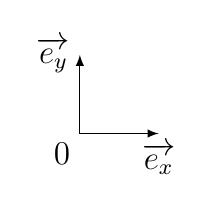
\begin{tikzpicture}[>= latex]
\draw [->] (0, 0) node[anchor= north east] {$0$} -- (0, 1)
node [anchor=east] {$\vec{e_{y}}$};
\draw [->] (0, 0) -- (1, 0) node [anchor=north] {$\vec{e_{x}}$};
\end{tikzpicture}
\end{center}

\item  Repère oblique ($0, \vec{e_{x}}, \vec{e_{y}}$)
\begin{center}
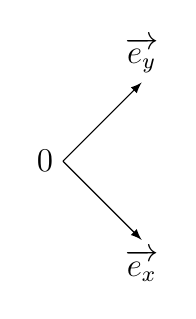
\begin{tikzpicture}[>= latex]
\draw [->] (0, 0) node[anchor= east] {$0$} -- (1, 1)
node [anchor=south] {$\vec{e_{y}}$};
\draw [->] (0, 0) -- (1, -1) node [anchor=north] {$\vec{e_{x}}$};
\end{tikzpicture}
\end{center}
\end{itemize}

\Warning référentiel (physique: \textbf{réel})  $\iff$ repère (géométrique:
\textbf{virtuel}) \Warning

\section{Vecteur position et déplacements}
\label{sec:vecteur_position_et_deplacements}

\subsection{Vecteur position}
\label{sub:vecteur_position}

\begin{itemize}
\item La position d'un objet (point materiel) dans le référentiel est
donné par le vecteur position $\vec r$:
\begin{center}
\includegraphics[width=5cm]{fig1}
\end{center}

\item Unité physique (SI): mètre [ m ]
\end{itemize}

\paragraph{Vecteur}
\label{par:vecteur}

Un vecteur possède 3 propriétés fondamentale:

\begin{itemize}
\item Direction
\item Sens
\item Norme
\end{itemize}

On le note par un symbole surmonté d'une flèche (manuscrit) ou en gras
(caractère d'imprimerie)

Pour le vecteur position \textbf{r}, la \textbf{direction} est la droite
passant pas $O$ et l'objet, le \textbf{sens} est donné par le regard vers
l'objet depuis $O$ et la \textbf{norme} par la distance de $O$ à l'objet.

\begin{itemize}
\item Le vecteur position $\vec r$ peut être décomposé dans le repère orthonormée
$(O, \vec{e_{x}}, \vec{e_{y}})$

\begin{center}
\includegraphics[width=5cm]{fig2.png}
\end{center}

\item Vecteur position $\vec r$:

\begin{equation}
\vec r = x \cdot \vec{e_{x}} + y \cdot \vec{e_{y}} = \myVector{x}{y}{}
= \myVector{\cos(\alpha)\cdot r}{\sin(\alpha)\cdot r}{}
\end{equation}

$$ \textrm{où}\ r = \| \vec r \| = \sqrt{x^{2} + y^{2}}$$
         
$x$ et $y$ sont les \textbf{composants} du vecteurs position $\vec r$
dans le repère orthonormée $(O, \vec{e_{x}}, \vec{e_{y}})$

\item Comme l'objet peut se déplacer au cours du temps, sa position peut
changer.
\end{itemize}

\subsection{Temps}
\label{sub:temps}

Temps ($t$ ou $T$): grandeurs scalaire qui décrit l'évolution d'un système
physique.

\begin{itemize}
\item Unité physique (SI): secondes [ s ]

\item Comme un objet se déplace au cours du temps, son vecteur position
est function du temps: $\vec r \equiv \vec r (t)$

\item Vecteur position à l'instant $t$:

\begin{equation}
\vec r (t) = x(t) \cdot \vec{e_{x}} + y(t) \cdot \vec{e_{y}} =
\myVector{x(t)}{y(t)}{} = \myVector{r(t) \cdot \cos(\alpha(t))}{r(t) \cdot \sin(\alpha(t))}{}
\end{equation}

\item \textbf{Exemples}: horaires de train (Où? Quand?), GPS
\end{itemize}

\subsection{Trajectoire}
\label{sub:trajectoire}

\begin{itemize}
\item Lieux géométrique des points de l'espace occupés par l'objet (point
matériel) au cours du temps.

\pagebreak

\item Ensemble des points qui sont atteints par l'objet (courbe ou droite)
représenté par $\Gamma$

\begin{center}
\includegraphics[width=8cm]{fig3}
\end{center}
\end{itemize}


$$\Gamma = \{ P | \exists t, \vec{OP} = \vec r (t)\}$$

\paragraph{Exemples}
\label{par:exemples}

\begin{enumerate}
\item Droite (chute libre)
\item Cercle (electron dans un champ magnétique)
\item Parabole (projectile)
\item Ellipse (planète)
\item Hyperbole (astéroïde)
\end{enumerate}

La trajectoire répond à la question "où?" sans se préoccuper de la question
"quand?".

\pagebreak

\subsection{Déplacement}
\label{sub:deplacement}

Le vecteur déplacement est la variation du vecteur position au cours du temps.
On considère les position $P_{1}$ et $P_{2}$ d'un objet aux temps $t_{1}$ et $t_{2}$
où $t_{1} < t_{2}$.

\begin{center}
\includegraphics[width=8cm]{fig4}
\end{center}

$$\vec{r_{1}} + \Delta \vec r = \vec{r_{2}}$$

\begin{itemize}
\item Déplacement le long de 
\begin{equation}
\Gamma: \Delta \vec r = \vec{r_{2}} - \vec{r_{1}} = \vec r (t_{1}) - \vec r (t_{1})
\end{equation}

\item \textbf{Exemple}: Le vecteur déplacement $\Delta \vec r$ entre
Genève (position $\vec{r_{1}}$) et Lausanne (position $\vec{r_{2}}$) le
long des voies le chemin de fer (trajectoire $\Gamma$)
\end{itemize}

\paragraph{Cas particuliers:}
\label{par:cas_particuliers_}

\begin{enumerate}
\item Objet immobile au point $A$

\begin{center}
\includegraphics[width=5cm]{fig5}
\end{center}

Vecteur position indépendant du temps $t$: 

\begin{equation}
\label{eq:rt_cste}
\vec r (t) = \vec{OA} = \vec{r_{0}} = \vec{cste} \quad \forall t
\end{equation}

\item Objet qui avance régulièrement  sur une droite $\Gamma$ qui passe
par un point $A$ l'instant $t_{0}: \vec r (t_{0}) = \vec{OA} =
\vec{r_{0}}$

\begin{center}
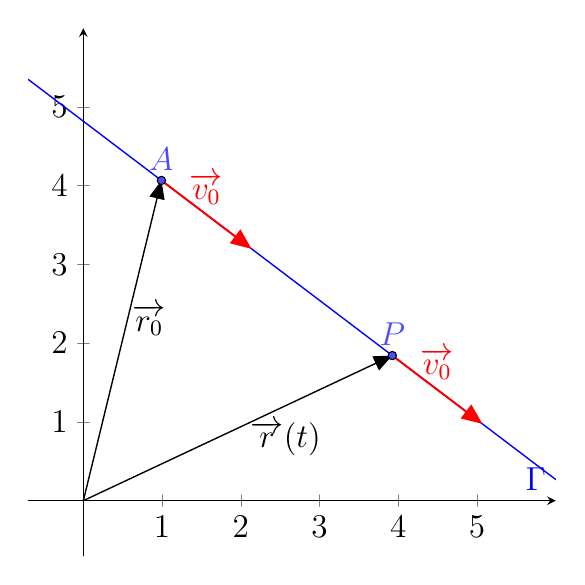
\begin{tikzpicture}[line cap=round,line join=round,>=triangle 45,x=1.0cm,y=1.0cm]
\begin{axis}[
x=1.0cm,y=1.0cm,
axis lines=middle,
xmin=-0.7,
xmax=6.0,
ymin=-0.7,
ymax=6.0,
xtick={0.0,1.0,...,5.0},
ytick={0.0,1.0,...,5.0},]
\clip(-0.7,-0.7) rectangle (6.,6.);
\draw [->,line width=0.5pt] (0.,0.) -- (0.9912936274413515,4.066851325623913) node [anchor=south,color=ududff] {$A$};
\draw [->,line width=0.5pt] (0.,0.) -- (3.9237546376441306,1.8428441986199695) node [anchor=south,color=ududff] {$P$};
\draw [line width=0.5pt,color=qqqqff,domain=-0.7:6.] plot(\x,{(--14.13052703906677-2.2240071270039437*\x)/2.932461010202779}) node [anchor = east]{$\Gamma$};
\draw [->,line width=0.7pt,color=ffqqqq] (0.9912936274413515,4.066851325623913) -- (2.1358112820513946,3.1988379361948893) node [color=ffqqqq, midway,anchor=south] {$\vec{v_{0}}$};
\draw [->,line width=0.7pt,color=ffqqqq] (3.9237546376441306,1.8428441986199695) -- (5.068272292254173,0.9748308091909454) node [color=ffqqqq, midway,anchor=south] {$\vec{v_{0}}$};
\begin{scriptsize}
\draw [fill=ududff] (0.9912936274413515,4.066851325623913) circle (1.5pt);
\draw[color=black] (0.5025501257408889,2.2912327322901245) node [anchor=west] {$\vec{r_{0}}$};
\draw [fill=ududff] (3.9237546376441306,1.8428441986199695) circle (1.5pt);
\draw[color=black] (2.5696212659602815,0.7891311444951222) node {$\vec r(t)$};
\draw[color=qqqqff] (-0.11174216538721699,4.555594827324382) ;
\end{scriptsize}
\end{axis}
\end{tikzpicture}
\end{center}

\begin{itemize}
\item Le vecteur déplacement $\Delta \vec r = \vec r (t) -
\vec{r_{0}}$ est proportionnelle à sa durée $\Delta t = t -
t_{0}$

\item Il existe un vecteur directeur $\vec{v_{0}}$ de la droite
tel que $\Delta \vec r = \vec{v_{0}} \cdot \Delta t$, ou
encore 

\begin{equation}
\vec r (t) = \vec{v_{0}} \cdot (t - t_{0}) + \vec{r_{0}} 
\label{eq:2.7}
\end{equation}
\end{itemize}

\item L'objet est dit en mouvement rectiligne uniforme (MRU)

\item Dans le plan, on donne l'origine $O$ et un point $A$. Un objet
se déplace de $O$ à $A$ entre $t = 0$ et $t = t_{A}$

\item On cherche à déterminer l'équation horaire $\vec r (t)$ de
l'objet en considérant que celui-ci passe en $O$ à l'instant $t =
0$.

\begin{center}
\includegraphics[width=8cm]{fig7}
\end{center}

\item Conditions l'initiale et finale: $\vec r (0) = \vec 0$ et $\vec
r (t_{A}) = \vec{OA}$

\item Ainsi: 
\begin{equation}
\vec r (t_{A}) = \vec{v_{0}} \cdot t_{A} = \vec{OA} \implies
\vec{v_{0}} = \frac{\vec{OA}}{t_{A}}
\end{equation}

\item Finalement, \begin{equation}\vec r (t) = \vec{v_{0}} \cdot t = \frac{t}{t_{A}}
\cdot \vec{OA}\end{equation}

\item \textbf{Rencontre}: Lorsque deux objets se trouvent à la même
position au même temps $t_{r}$, il y a rencontre

\begin{equation}
\exists t_{r} \vec{r_{1}} (t_{1}) = \vec{r_{2}} (t_{r})
\end{equation}
\end{enumerate}

\section{Vecteur vitesse}
\label{sec:vecteur_vitesse}

\subsection{Vitesse moyenne}
\label{sub:vitesse_moyenne}

On considère un objet en position initiale $P_{1}$ au temps initiale $t_{1}$
et en position finale $P_{2}$ au temps finale $t_{2}$

\begin{center}
\includegraphics[width=8cm]{fig4}
\end{center}

\begin{itemize}
\item Position initiale: $\vec{r_{1}} = \vec r (t_{1})$
\item Position finale: $\vec{r_{2}} = \vec r (t_{2})$
\item Déplacement: $\Delta \vec r = \vec{r_{2}} - \vec{r_{1}}$
\item Intervalle de temps: $\Delta t = t_{2} - t_{1}$
\end{itemize}


\begin{itemize}
\item La \textbf{vitesse moyenne} ($\vec{v_{moy}}$) de l'objet est définie
comme le rapport entre le déplacement $\Delta \vec r$ et l'intervalle
de temps $\Delta t$

\begin{equation}
\vec{v_{moy}} = \frac{\Delta \vec r}{\Delta t} 
\end{equation}

\item Unité physique (SI): mètre par secondes 
[ $\frac{\textrm{m}}{\textrm{s}}$ ]

\item La vitesse moyenne ne donne que la position finale $\vec{r_{2}}$ par
rapport à la position initiale $\vec{r_{1}}$ et non les positions
intermédiaires 

\begin{equation}
\vec{r_{2}} = \vec{r_{1}} + \vec{v_{moy}} \cdot \Delta t
\end{equation}
        
\item C'est  la vitesse constante qu'il faudrait maintenir pour faire le
déplacement $\Delta \vec r$ durant l'intervalle du temps $\Delta t$.
\end{itemize}

\begin{center}
\begin{minipage}{.5\linewidth}
\resizebox{\textwidth}{!}{
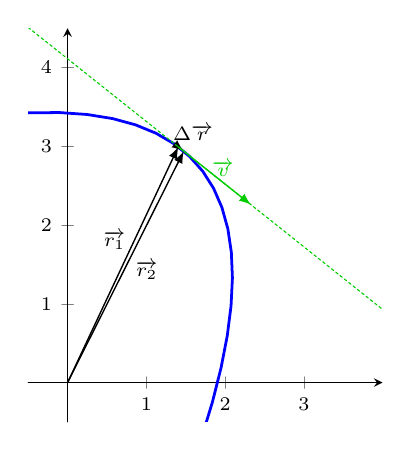
\begin{tikzpicture}[line cap=round,line join=round, >= latex,x=1.0cm,y=1.0cm]
\tikzstyle{every node}=[font=\scriptsize]
\begin{axis}[
x=1.0cm,y=1.0cm,
axis lines=middle,
xmin=-0.5,
xmax=4.0,
ymin=-0.5,
ymax=4.5,
xtick={-0.0,1.0,...,3.0},
ytick={-0.0,1.0,...,4.0},]
\clip(-0.5,-0.5) rectangle (4.,5.);
\draw [samples=50,rotate around={-228.3882158815608:(1.63721103787723,2.780353297122578)},xshift=1.63721103787723cm,yshift=2.780353297122578cm,line width=1pt,color=qqqqff,domain=-6.184162744813402:6.184162744813402)] plot (\x,{(\x)^2/2/1.5460406862033504});
\draw [->,line width=.5pt] (0.,0.) -- (1.4054298862371315,2.993507684986792);
\draw [->,line width=.5pt] (0.,0.) -- (1.475367905161338,2.9378595326316175);
\draw [->,line width=.5pt] (1.4054298862371315,2.993507684986792) -- (1.475367905161338,2.9378595326316175);
\draw [dash pattern=on 1pt off 1pt,color=qqccqq,domain=-0.5:4.] plot(\x,{(--0.28756957355620383-0.055648152355174396*\x)/0.06993801892420648});
\draw [->,line width=0.5pt,color=qqccqq] (1.4054298862371315,2.993507684986792) -- (2.3295147609991482,2.2582335566818714);
\draw[color=black] (0.598112073142613,1.8097492393092884) node {$\vec{r_{1}}$};
\draw[color=black] (1.006788281285858,1.427564527508181) node {$\vec{r_{2}}$};
\draw[color=black] (1.5949506619244465,3.1712822751007335) node {$\Delta \vec r$};
\draw[color=qqccqq] (1.9760136127607153,2.7140255663386945) node {$\vec v$};
\end{axis}
\end{tikzpicture}
}
\end{minipage}
\begin{minipage}{.49\linewidth}
\begin{itemize}
\item Dans la limite où l'intervalle de $\Delta t$ est très petit,
le déplacement 
\begin{equation}\Delta \vec r = \vec{r_{2}} - \vec{r_{1}}\end{equation}
donne la direction et le sens de mouvement est juste après le
temps $t_{1}$.
\item Le déplacement $\Delta \vec r$ devient vecteur directeur de
la tangente à la trajectoire en $\vec{r_{0}}$ 
\end{itemize}
\end{minipage}
\end{center}

\begin{itemize}
\item La \textbf{vitesse instantanée} ou \textbf{vitesse} de l'objet est
définie comme la vitesse moyenne dans la limite d'un intervalle du
temps infinitésimale.

\begin{equation}
\label{eq:2.13}
\vec v (t) = \lim_{\Delta t \to 0} \frac{\Delta \vec r}{\Delta t}
= \lim_{\Delta t \to 0} \frac{\vec r (t + \Delta t) - \vec r (t)}{\Delta t}
= \frac{d\vec r}{dt} = \dot{\vec r} (t)
\end{equation}
\end{itemize}

\paragraph{Propriétés de la vitesse}
\label{par:proprietes_de_la_vitesse}

\markDate{6/03/2019}


\begin{itemize}
\item Taux de variation de la position par rapport au temps (dérivée)
\item Vector (direction, sens, norme)
\item Tangente à la trajectoire dans le sens du mouvement
\end{itemize}



\paragraph{Cas particuliers}

\begin{enumerate}
\item Objet immobile qui se trouve au point A

\begin{center}
\begin{minipage}{.5\linewidth}
\resizebox{\textwidth}{!}{
\begin{tikzpicture}[line cap=round,line join=round,>=triangle 45,x=1.0cm,y=1.0cm]
\begin{axis}[
x=1.0cm,y=1.0cm,
axis lines=middle,
xmin=-0.5,
xmax=5.9,
ymin=-0.19595529090418443,
ymax=5.656623567248618,
xtick={-0.0,1.0,...,5.0},
ytick={-0.0,1.0,...,5.0},]
\clip(-0.5,-0.19595529090418443) rectangle (5.9,5.656623567248618);
\draw [->,] (0.,0.) -- (5.213746581801192,4.798140383149461) node[midway,
anchor= south east] {$\vec r_{0}$};
\begin{scriptsize}
\draw [fill=ududff] (5.213746581801192,4.798140383149461) circle (1.5pt) node[anchor=south] {$A$};
\draw[color=ududff] (5.347619047619048,4.896413146171829);
\draw[color=black] (2.3,2.601896761095316) ;
\end{scriptsize}
\end{axis}
\end{tikzpicture}
}
\end{minipage}
\begin{minipage}{.4\linewidth}
Vecteur vitesse nulle (position constante):
\begin{equation}
\vec v(t) = \vec 0, \quad \forall t
\end{equation}
$$ \text{ car } \vec r (t) = \vec{0A} = \vec{r_{0}} \quad (\ref{eq:rt_cste})$$
\end{minipage}
\end{center}

\paragraph{Vérification:}
\label{par:verification}

$$\vec v (t) = \lim_{\Delta t \to 0} \frac{\vec r ( t + \Delta t) - \vec r (t)}{\Delta t} 
= \lim_{\Delta t \to 0} \frac{\vec{r_{0}} - \vec{r_{0}}}{\Delta t} = \vec 0 $$

\cqfd
\item Objet qui avance  à vitesse constante 

\begin{center}
\begin{minipage}{.5\linewidth}
\resizebox{\textwidth}{!}{
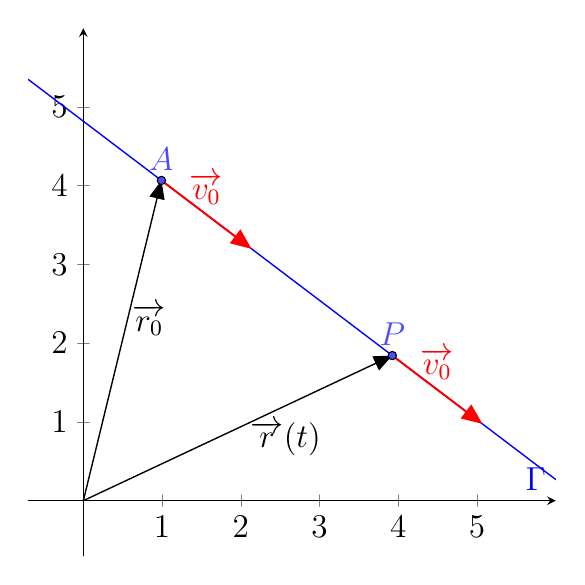
\begin{tikzpicture}[line cap=round,line join=round,>=triangle 45,x=1.0cm,y=1.0cm]
\begin{axis}[
x=1.0cm,y=1.0cm,
axis lines=middle,
xmin=-0.7,
xmax=6.0,
ymin=-0.7,
ymax=6.0,
xtick={0.0,1.0,...,5.0},
ytick={0.0,1.0,...,5.0},]
\clip(-0.7,-0.7) rectangle (6.,6.);
\draw [->,line width=0.5pt] (0.,0.) -- (0.9912936274413515,4.066851325623913) node [anchor=south,color=ududff] {$A$};
\draw [->,line width=0.5pt] (0.,0.) -- (3.9237546376441306,1.8428441986199695) node [anchor=south,color=ududff] {$P$};
\draw [line width=0.5pt,color=qqqqff,domain=-0.7:6.] plot(\x,{(--14.13052703906677-2.2240071270039437*\x)/2.932461010202779}) node [anchor = east]{$\Gamma$};
\draw [->,line width=0.7pt,color=ffqqqq] (0.9912936274413515,4.066851325623913) -- (2.1358112820513946,3.1988379361948893) node [color=ffqqqq, midway,anchor=south] {$\vec{v_{0}}$};
\draw [->,line width=0.7pt,color=ffqqqq] (3.9237546376441306,1.8428441986199695) -- (5.068272292254173,0.9748308091909454) node [color=ffqqqq, midway,anchor=south] {$\vec{v_{0}}$};
\begin{scriptsize}
\draw [fill=ududff] (0.9912936274413515,4.066851325623913) circle (1.5pt);
\draw[color=black] (0.5025501257408889,2.2912327322901245) node [anchor=west] {$\vec{r_{0}}$};
\draw [fill=ududff] (3.9237546376441306,1.8428441986199695) circle (1.5pt);
\draw[color=black] (2.5696212659602815,0.7891311444951222) node {$\vec r(t)$};
\draw[color=qqqqff] (-0.11174216538721699,4.555594827324382) ;
\end{scriptsize}
\end{axis}
\end{tikzpicture}
}
\end{minipage}
\begin{minipage}{.49\linewidth}
\begin{itemize}
\item Vecteur de vitesse constant 
\begin{equation}
\vec v (t) = \vec{v_{0}} = \vec{cste}
\end{equation}
\item Vitesse et vitesse moyenne identiques
$$ \vec r (t) = \vec{V_{0}} \cdot (t-t_{0}) +
\vec{r_{0}} \quad \eqref{eq:2.7} $$
\end{itemize}
\end{minipage}
\end{center}

Mouvement rectiligne uniforme  à vitesse constante (MRU).

            
\paragraph{Vérification}
$\vec v (t) \stackbin[\eqref{eq:2.13}]{\eqref{eq:2.7}}{=} \lim_{\Delta
t \to 0} \frac{\vec v  (t + \Delta t - t_{0}) + \vec{r_{0}} -
\vec v (t - t_{0}) - \vec{r_{0}}}{\Delta t} = \vec{V_{0}}$

\item Objet qui passe par $A$ l'instant $t_{0}$, i.e. $\vec r (t) =
\vec{OA} = \vec{r_{0}}$, avec une vitesse $\vec{v_{0}}$, et dont la
vitesse change régulièrement.

\begin{center}
\begin{minipage}{.5\linewidth}
\resizebox{\textwidth}{!}{
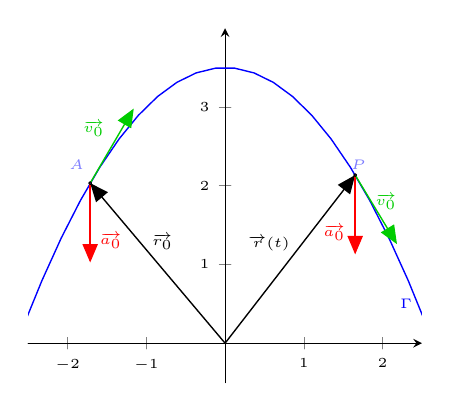
\begin{tikzpicture}[line cap=round,line join=round,>=triangle 45,x=1.0cm,y=1.0cm]
\tikzstyle{every node}=[font=\tiny]
\begin{axis}[
x=1.0cm,y=1.0cm,
axis lines=middle,
xmin=-2.5,
xmax=2.5,
ymin=-0.5,
ymax=4.0,
xtick={-2.0,-1.0,...,2.0},
ytick={-0.0,1.0,...,3.0},]
\clip(-2.5,-0.5) rectangle (2.5,4.);
\draw [samples=50,rotate around={-180.:(0.,3.5)},xshift=0.cm,yshift=3.5cm,line width=.5pt,color=qqqqff,domain=-5.999999999999998:5.999999999999998)] plot (\x,{(\x)^2/2/0.9999999999999998});
\draw [->,line width=.5pt] (0.,0.) -- (-1.7133327095990474,2.032245513108993);
\draw [->,line width=.5pt] (0.,0.) -- (1.6521556070681371,2.1351909250166576);
\draw [->,line width=.5pt,color=ffqqqq] (-1.7133327095990474,2.032245513108993) -- (-1.7133327095990474,1.02491) node [midway, anchor=north west] {$\vec{a_{0}}$};
\draw [->,line width=.5pt,color=ffqqqq] (1.6521556070681371,2.1351909250166576) -- (1.6521556070681371,1.1278554119076645) node [midway, anchor= north east] {$\vec{a_{0}}$};
\draw [->,line width=.5pt,color=qqccqq] (-1.7133327095990474,2.032245513108993) -- (-1.1601772404679775,2.9799848718648616);
\draw [->,line width=.5pt,color=qqccqq] (1.6521556070681371,2.1351909250166576) -- (2.182824625954755,1.2584431299657848);
\draw [color=qqqqff] (2.3, .5) node {$\Gamma$};
\draw [fill=xdxdff] (-1.7133327095990474,2.032245513108993) circle (.5pt);
\draw[color=xdxdff] (-1.8853238772020617,2.2604914359383574) node {$A$};
\draw [fill=xdxdff] (1.6521556070681371,2.1351909250166576) circle (.5pt);
\draw[color=xdxdff] (1.6933542697820383,2.2604914359383574) node {$P$};
\draw[color=black] (-0.7946002135765065,1.2879678389444655) node {$\vec{r_{0}}$};
\draw[color=black] (0.942273671032289,1.2709060214533447) node [anchor=east] {$\vec r (t)$};
\draw[color=qqccqq] (-1.6671791444769506,2.721160508198622) node {$\vec{v_{0}}$};
\draw[color=qqccqq] (2.0440426375806346,1.7929976366816445) node {$\vec{v_{0}}$};
\end{axis}
\end{tikzpicture}
}
\end{minipage}
\begin{minipage}{.49\linewidth}
\begin{itemize}
\item La variation de vitesse $$\Delta \vec v = \vec v (t) - \vec{v_{0}} $$
est proportionnellement à la durée $$\Delta \vec t = t
- t_{0}$$
\item Il existe un vecteur $\vec{a_{0}}$ tel que $$\Delta
\vec v = \vec{a_{0}} \cdot \Delta t$$
\end{itemize}
\end{minipage}
\end{center}
\end{enumerate}

Ainsi, 
\begin{equation}
\label{eq:2.17}
\vec v (t) = \vec{a_{0}} \cdot (t - t_{0}) + \vec{v_{0}} 
\end{equation}

\begin{itemize}
\item Mouvement uniformément accéléré (MUA) \eqref{eq:2.17}
\item Le vecteur position $\vec r (t)$ s'écrit:
\begin{equation}
\vec r (t) = \frac{1}{2} \cdot (t - t_{0})^{2} + \vec{v_{0}} \cdot
(t - t_{0}) + \vec{r_{0}} 
\end{equation}
\end{itemize}

\section{Vecteur accélération}
\label{sec:vecteur_acceleration}

\subsection{Accélération moyenne}
\label{sub:acceleration_moyenne}

On considère un objet en position initiale $P_{1}$ au temps initiale $t_{1}$ et
en position finale $P_{2}$ au temps finale $t_{2}$.

\begin{center}
\begin{minipage}{.5\linewidth}
\resizebox{\textwidth}{!}{
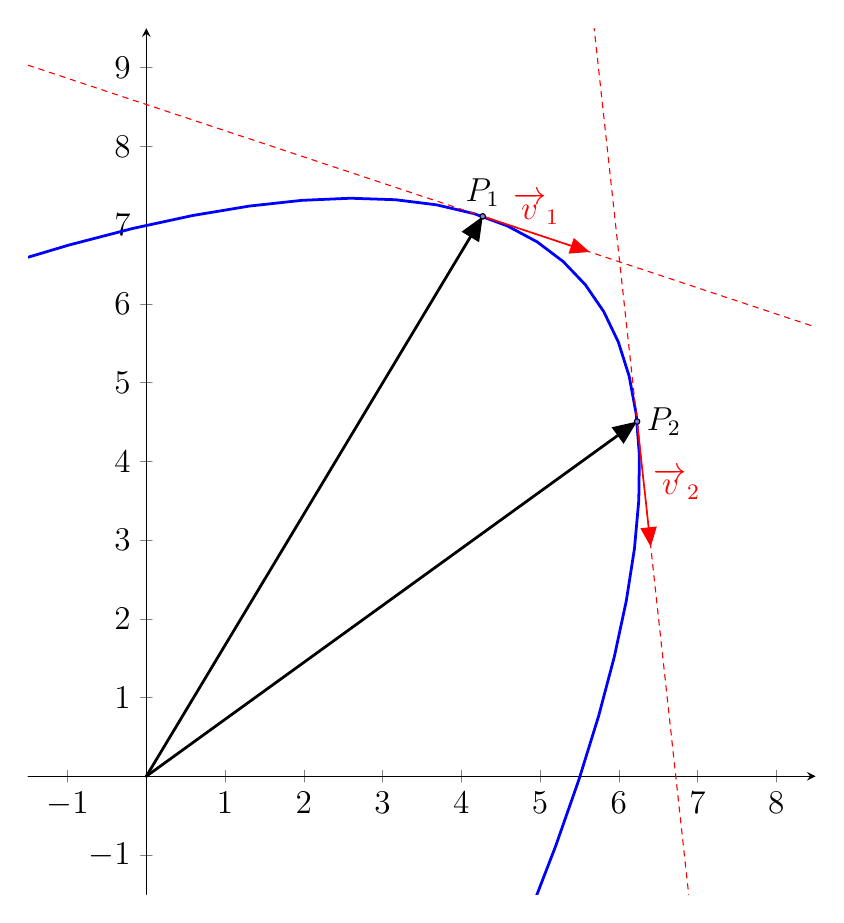
\begin{tikzpicture}[line cap=round,line join=round,>=triangle 45,x=1.0cm,y=1.0cm]
\begin{axis}[
x=1.0cm,y=1.0cm,
axis lines=middle,
xmin=-1.5,
xmax=8.5,
ymin=-1.5,
ymax=9.5,
xtick={-1.0,0.0,...,8.0},
ytick={-1.0,0.0,...,9.0},]
\clip(-1.5,-1.5) rectangle (8.5,9.5);
\draw [samples=50,rotate around={-226.3239152314405:(5.440788291375457,6.394952040437883)},xshift=5.440788291375457cm,yshift=6.394952040437883cm,line width=1pt,color=qqqqff,domain=-9.992404550973422:9.992404550973422)] plot (\x,{(\x)^2/2/2.4981011377433555});
\draw [->,line width=1pt] (0.,0.) -- (4.272178987631289,7.110416256476802);
\draw [->,line width=1pt] (0.,0.) -- (6.23214433544671,4.505182789489529);
\draw [dash pattern=on 2pt off 2pt,color=ffqqqq,domain=-1.5:8.5] plot(\x,{(--234.21463243508686-9.128549587427678*\x)/27.45490948188976});
\draw [->,line width=0.6pt,color=ffqqqq] (4.272178987631289,7.110416256476802) -- (5.630428061706034,6.658808720383931)node [midway, anchor=south] {$\vec v_1$};
\draw [line width=0.4pt,dash pattern=on 2pt off 2pt,color=ffqqqq,domain=-1.5:8.5] plot(\x,{(--215.2147337277429-32.0080211935226*\x)/3.4928939607921663});
\draw [->,line width=0.6pt,color=ffqqqq] (6.23214433544671,4.505182789489529) -- (6.405724674727298,2.9145352517063223)node [midway, anchor=west] {$\vec v_2$};
\begin{scriptsize}
\draw [fill=xdxdff] (4.272178987631289,7.110416256476802) circle (1pt) node [anchor=south]{$P_1$};
\draw [fill=xdxdff] (6.23214433544671,4.505182789489529) circle (1pt)node [anchor=west]{$P_2$};
\end{scriptsize}
\end{axis}
\end{tikzpicture}
}
\end{minipage}
\begin{minipage}{.49\linewidth}
\begin{itemize}
\item Vitesse initiale: $\vec{v_{1}} = \vec v (t_{1})$ 
\item Vitesse finale: $\vec{v_{2}} = \vec v (t_{2})$ 
\item Variation de vitesse: $\Delta \vec v = \vec{v_{2}} - \vec{v_{1}}$ 
\item Intervalle de temps: $\Delta t = t_{2} - t_{1}$ 
\end{itemize}
\end{minipage}
\end{center}

\begin{itemize}
\item L'\textbf{accélération moyenne} $\vec{a_{moy}}$ est définie comme
le rapport entre la variation de la vitesse $\Delta \vec v$ et
l'intervalle $\Delta t$ 
\begin{equation}
\vec{a_{moy}} = \frac{\Delta \vec v}{\Delta t}
\end{equation}
\item Unité physique (SI): mètres par secondes \big[$\frac{m}{s^{2}}$\big]
\item L'accélération moyenne donne que la vitesse finale $\vec{v_{2}}$ par
rapport à la vitesse initiale $\vec{v_{1}}$ et non les vitesses
intermédiaire
\begin{equation}
\vec{v_{2}} = \vec{v_{1}} + \vec{a_{moy}} \cdot t
\end{equation}

\item C'est l'accélération constante qu'il faudrait maintenir pour
effectuer une variation de vitesse $\Delta \vec v$ en un intervalle de
temps $\Delta t$ 

\begin{center}
\begin{minipage}{.5\linewidth}
\resizebox{\textwidth}{!}{
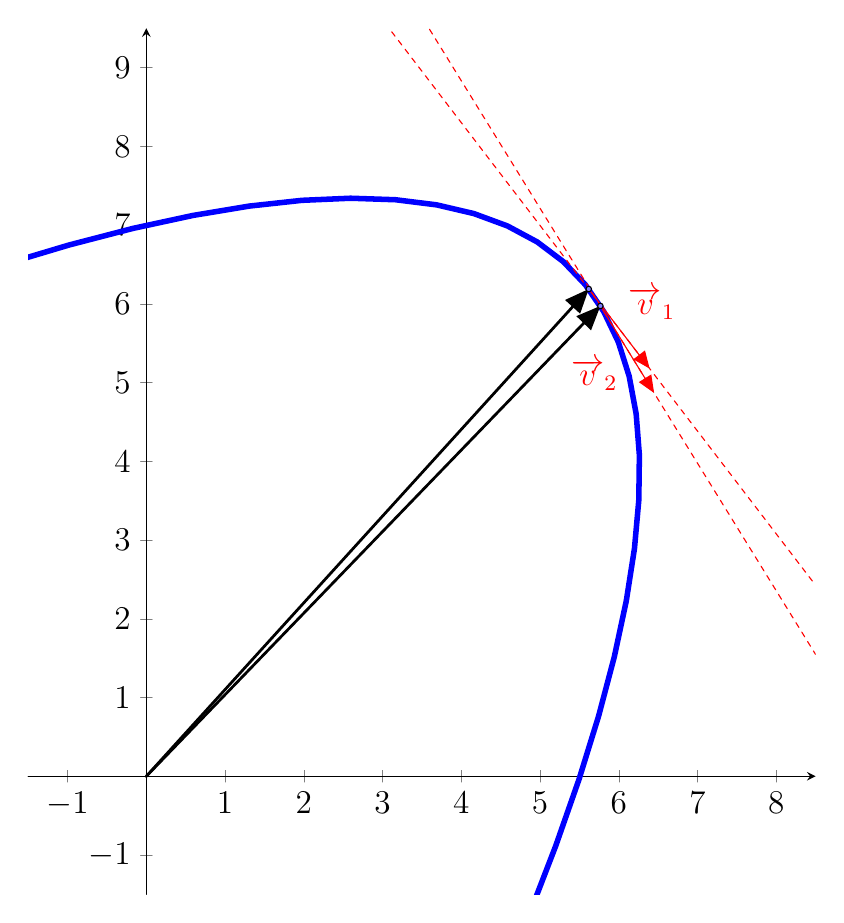
\begin{tikzpicture}[line cap=round,line join=round,>=triangle 45,x=1.0cm,y=1.0cm]
\begin{axis}[
x=1.0cm,y=1.0cm,
axis lines=middle,
xmin=-1.5,
xmax=8.5,
ymin=-1.5,
ymax=9.5,
xtick={-1.0,0.0,...,8.0},
ytick={-1.0,0.0,...,9.0},]
\clip(-1.5,-1.5) rectangle (8.5,9.5);
\draw [samples=50,rotate around={-226.3239152314405:(5.440788291375457,6.394952040437883)},xshift=5.440788291375457cm,yshift=6.394952040437883cm,line width=2.pt,color=qqqqff,domain=-9.992404550973422:9.992404550973422)] plot (\x,{(\x)^2/2/2.4981011377433555});
\draw [->,line width=1.pt] (0.,0.) -- (5.618304144219443,6.187494013986672);
\draw [->,line width=1.pt] (0.,0.) -- (5.766158881810352,5.972757821180305);
\draw [line width=0.4pt,dash pattern=on 2pt off 2pt,color=ffqqqq,domain=-1.5:8.5] plot(\x,{(--211.43612782220725-20.41448267396259*\x)/15.634981624920506});
\draw [->,line width=0.4pt,color=ffqqqq] (5.618304144219443,6.187494013986672) -- (6.391797836822294,5.17754888166289) node [midway, anchor = south west]{$\vec v_1$};
\draw [line width=0.4pt,dash pattern=on 2pt off 2pt,color=ffqqqq,domain=-1.5:8.5] plot(\x,{(--210.20725053878897-22.23348934383533*\x)/13.729908518037238});
\draw [->,line width=0.4pt,color=ffqqqq] (5.766158881810352,5.972757821180305) -- (6.448470513827898,4.867858369031175) node [midway, anchor = north east]{$\vec v_2$};
\begin{scriptsize}
\draw [fill=xdxdff] (5.618304144219443,6.187494013986672) circle (1pt);
\draw [fill=xdxdff] (5.766158881810352,5.972757821180305) circle (1pt);
\draw[color=ffqqqq] (0.7359655472418168,12.755156905856063) node {$g$};
\draw[color=ffqqqq] (1.7148041199644106,12.755156905856063) node {$h$};
\end{scriptsize}
\end{axis}
\end{tikzpicture}
}
\end{minipage}
\begin{minipage}{.49\linewidth}
\setlength{\parskip}{.3em}
Dans la limite où l'intervalle de temps $\Delta t$
est très petit, la variation de vitesse $\Delta \vec v
= \vec{v_{2}} - \vec{v_{1}}$ donne la direction et le
sens de l'accélération juste après $t_{1}$.
\vspace{1cm}

Le vecteur variation de vitesse $\Delta \vec v$ devient le
vecteur directeur de l'accélération.
\end{minipage}
\end{center}

\item L'\textbf{accélération instantanée} ou \textbf{accélération} de
l'objet est déterminé comme l'accélération moyenne dans la limite d'un
intervalle de temps infinitésimale.

\begin{equation}
\label{eq:2.21}
\vec a (t) = \lim_{\Delta t \to 0}  \frac{\Delta \vec v}{\Delta t}
\end{equation}

\begin{equation}
\implies \lim_{\Delta t \to 0} \frac{\vec v (t+\Delta t) - \vec v
(t)}{\Delta t} = \frac{d\vec v}{dt} = \vec v (t)
\end{equation}
\end{itemize}

\paragraph{Propriétés de l'accélération}

\begin{itemize}
\item Taux de variation de la variation vitesse par rapport au temps (dérivée)
\item Vecteur (direction, sens, norme)
\item Toujours dirigée vers l'intérieur de la trajectoire (courbe)
\item Selon la tangente à la trajectoire le vecteur accélération va
décrire un changement de norme du vecteur vitesse
\item Selon la normale à la tangente: changement de direction du vecteur
vitesse
\end{itemize}


\paragraph{Cas particuliers}
\label{par:cas_particuliers}

\begin{enumerate}
\item Objet qui avance à vitesse constante $\vec{v_{0}}$ et qui passe par
le point $A$ à l'instant $t_{0} : \vec r (t_{0}) = \vec{OA}  = \vec{r_{0}}$.
La vitesse est constante (MRU) et donc l'accélération est nulle.

\begin{center}
\begin{minipage}{.5\linewidth}
\resizebox{\textwidth}{!}{
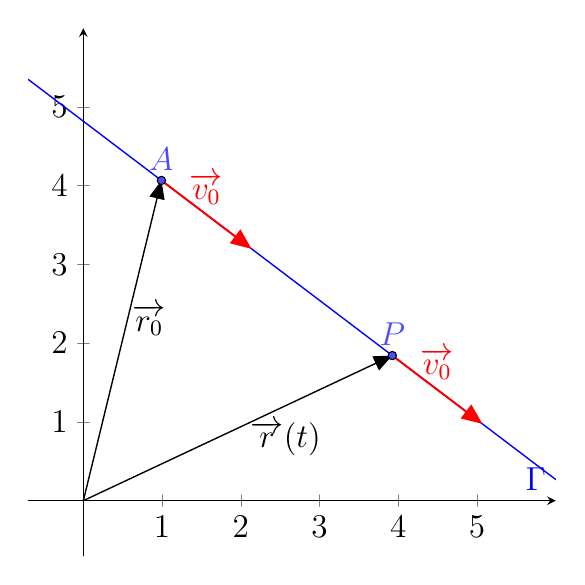
\begin{tikzpicture}[line cap=round,line join=round,>=triangle 45,x=1.0cm,y=1.0cm]
\begin{axis}[
x=1.0cm,y=1.0cm,
axis lines=middle,
xmin=-0.7,
xmax=6.0,
ymin=-0.7,
ymax=6.0,
xtick={0.0,1.0,...,5.0},
ytick={0.0,1.0,...,5.0},]
\clip(-0.7,-0.7) rectangle (6.,6.);
\draw [->,line width=0.5pt] (0.,0.) -- (0.9912936274413515,4.066851325623913) node [anchor=south,color=ududff] {$A$};
\draw [->,line width=0.5pt] (0.,0.) -- (3.9237546376441306,1.8428441986199695) node [anchor=south,color=ududff] {$P$};
\draw [line width=0.5pt,color=qqqqff,domain=-0.7:6.] plot(\x,{(--14.13052703906677-2.2240071270039437*\x)/2.932461010202779}) node [anchor = east]{$\Gamma$};
\draw [->,line width=0.7pt,color=ffqqqq] (0.9912936274413515,4.066851325623913) -- (2.1358112820513946,3.1988379361948893) node [color=ffqqqq, midway,anchor=south] {$\vec{v_{0}}$};
\draw [->,line width=0.7pt,color=ffqqqq] (3.9237546376441306,1.8428441986199695) -- (5.068272292254173,0.9748308091909454) node [color=ffqqqq, midway,anchor=south] {$\vec{v_{0}}$};
\begin{scriptsize}
\draw [fill=ududff] (0.9912936274413515,4.066851325623913) circle (1.5pt);
\draw[color=black] (0.5025501257408889,2.2912327322901245) node [anchor=west] {$\vec{r_{0}}$};
\draw [fill=ududff] (3.9237546376441306,1.8428441986199695) circle (1.5pt);
\draw[color=black] (2.5696212659602815,0.7891311444951222) node {$\vec r(t)$};
\draw[color=qqqqff] (-0.11174216538721699,4.555594827324382) ;
\end{scriptsize}
\end{axis}
\end{tikzpicture}
}
\end{minipage}
\begin{minipage}{.49\linewidth}
\setlength{\parskip}{.3em}
\begin{itemize}
\item $\vec a (t) = \vec 0$
\item $\vec v (t) = \vec{v_{0}} \quad \quad~\refstepcounter{equation}(\theequation)
\label{eq:2.23}$
\item $\vec r (t) = \vec{v_{0}} (t \cdot t_{0}) + \vec{r_{0}}$ 
\end{itemize}
\end{minipage}
\end{center}

\paragraph{Vérification:}
        
$\vec a (t) = \lim\limits_{\Delta t \to 0} \frac{\vec v (\Delta t + t) - \vec v
(t)}{\Delta t} = \lim\limits_{\Delta t \to 0} \frac{\vec{v_{0}} - \vec{v_{0}}}{\Delta
t} = \vec 0$ 
\cqfd

\item Objet qui passe par le point $A$ l'instant $t_{0}: \vec r (t_{0}) =
\vec{OA} = \vec{r_{0}}$  avec vitesse $\vec{v_{0}} : \vec v (t_{0})$ et
dont l'accélération $\vec{a_{0}}$ est constante.

\begin{center}
\begin{minipage}{.5\linewidth}
\resizebox{\textwidth}{!}{
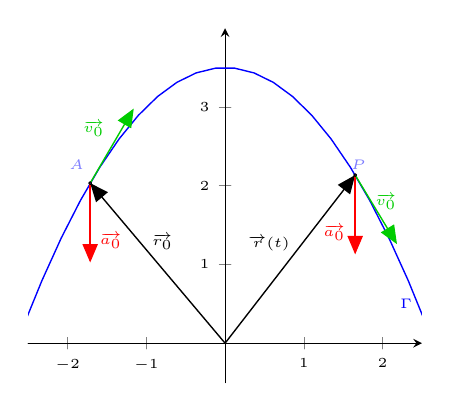
\begin{tikzpicture}[line cap=round,line join=round,>=triangle 45,x=1.0cm,y=1.0cm]
\tikzstyle{every node}=[font=\tiny]
\begin{axis}[
x=1.0cm,y=1.0cm,
axis lines=middle,
xmin=-2.5,
xmax=2.5,
ymin=-0.5,
ymax=4.0,
xtick={-2.0,-1.0,...,2.0},
ytick={-0.0,1.0,...,3.0},]
\clip(-2.5,-0.5) rectangle (2.5,4.);
\draw [samples=50,rotate around={-180.:(0.,3.5)},xshift=0.cm,yshift=3.5cm,line width=.5pt,color=qqqqff,domain=-5.999999999999998:5.999999999999998)] plot (\x,{(\x)^2/2/0.9999999999999998});
\draw [->,line width=.5pt] (0.,0.) -- (-1.7133327095990474,2.032245513108993);
\draw [->,line width=.5pt] (0.,0.) -- (1.6521556070681371,2.1351909250166576);
\draw [->,line width=.5pt,color=ffqqqq] (-1.7133327095990474,2.032245513108993) -- (-1.7133327095990474,1.02491) node [midway, anchor=north west] {$\vec{a_{0}}$};
\draw [->,line width=.5pt,color=ffqqqq] (1.6521556070681371,2.1351909250166576) -- (1.6521556070681371,1.1278554119076645) node [midway, anchor= north east] {$\vec{a_{0}}$};
\draw [->,line width=.5pt,color=qqccqq] (-1.7133327095990474,2.032245513108993) -- (-1.1601772404679775,2.9799848718648616);
\draw [->,line width=.5pt,color=qqccqq] (1.6521556070681371,2.1351909250166576) -- (2.182824625954755,1.2584431299657848);
\draw [color=qqqqff] (2.3, .5) node {$\Gamma$};
\draw [fill=xdxdff] (-1.7133327095990474,2.032245513108993) circle (.5pt);
\draw[color=xdxdff] (-1.8853238772020617,2.2604914359383574) node {$A$};
\draw [fill=xdxdff] (1.6521556070681371,2.1351909250166576) circle (.5pt);
\draw[color=xdxdff] (1.6933542697820383,2.2604914359383574) node {$P$};
\draw[color=black] (-0.7946002135765065,1.2879678389444655) node {$\vec{r_{0}}$};
\draw[color=black] (0.942273671032289,1.2709060214533447) node [anchor=east] {$\vec r (t)$};
\draw[color=qqccqq] (-1.6671791444769506,2.721160508198622) node {$\vec{v_{0}}$};
\draw[color=qqccqq] (2.0440426375806346,1.7929976366816445) node {$\vec{v_{0}}$};
\end{axis}
\end{tikzpicture}
}
\end{minipage}
\begin{minipage}{.49\linewidth}
\setlength{\parskip}{.3em}
\begin{itemize}
\item $\vec a (t) =  \vec{a_{0}} = \vec{cste}$
\item $\vec v (t) =  \vec{a_{0}} \cdot (t - t_{0}) +
\vec{v_{0}}\quad \quad~\refstepcounter{equation}(\theequation)
\label{eq:2.24}$
\item $\vec r (t) = \frac{1}{2} \cdot \vec{a_{0}} \cdot (t
- t_{0})^{2} + \vec{v_{0}} \cdot (t - t_{0}) + \vec{r_{0}}$ 
\end{itemize}
\end{minipage}
\end{center}

\paragraph{Vérification:}
        
$$\vec a (t) \stackbin[\eqref{eq:2.24}]{\eqref{eq:2.21}}{=}
\lim_{\Delta t \to 0} \frac{\vec{a_{0}} \cdot (t - \Delta t - t_{0}) +
\vec{v_{0}} - \vec{a_{0}} \cdot (t - t_{0}) - \vec{v_{0}}}{\Delta t} =
\vec{a_{0}}$$
\cqfd 
\end{enumerate}

On veut montrer que la trajectoire est une parabole d'axe verticale. On
choisit l'origine $O$ sur la trajectoire $\Gamma$ et l'origine du temps $t =
0$ lorsque l'objet passe en $O$. On prend prend $\vec{e_{x}}$ perpendiculaire
à $\vec{a_{0}}$ et $\vec{e_{y}}$ parallèle à $\vec{a_{0}}$.

\begin{center}
\begin{minipage}{.5\linewidth}
\resizebox{\textwidth}{!}{
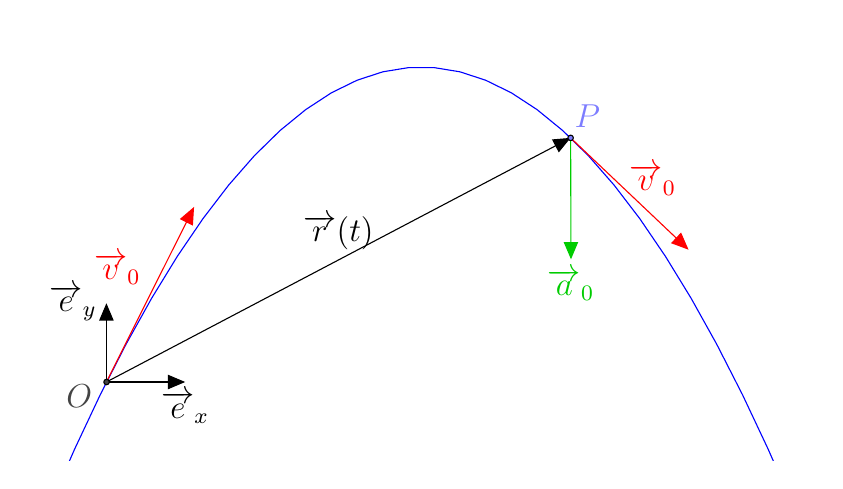
\begin{tikzpicture}[line cap=round,line join=round,>=triangle 45,x=1.0cm,y=1.0cm]
\clip(-1.,-1.) rectangle (9.,4.5);
\draw [samples=50,rotate around={-180.:(4.,3.9992768628452935)},xshift=4.cm,yshift=3.9992768628452935cm,line width=0.4pt,color=qqqqff,domain=-7.994214902762348:7.994214902762348)] plot (\x,{(\x)^2/2/1.998553725690587});
\draw [->,line width=0.4pt,color=ffqqqq] (0,0) -- (1.1133634707356288,2.2237141711451285) node [midway, anchor=south east]{$\vec v_0$};
\draw [->,line width=0.4pt] (0,0.) -- (0.,1.)node [anchor=east]{$\vec e_y$};
\draw [->,line width=0.4pt] (0,0.) -- (1.,0.) node [anchor=north]{$\vec e_x$};
\draw [->,line width=0.4pt] (0,0.) -- (5.895537446451206,3.1003612708570922) node [midway, anchor= south] {$\vec r (t)$};
\draw [->,line width=0.4pt,color=qqccqq] (5.895537446451206,3.1003612708570922) -- (5.9,1.55854) node [anchor=north]{$\vec a_0$};
\draw [->,line width=0.4pt,color=ffqqqq] (5.895537446451206,3.1003612708570922) -- (7.393075087098776,1.6800148279128146);
\draw [fill=uuuuuu] (0.0018079900265860363,0.) circle (1.0pt);
\draw[color=uuuuuu] (-0.3436358197316432,-0.17536988066984197) node {$O$};
\draw [fill=xdxdff] (5.895537446451206,3.1003612708570922) circle (1.0pt);
\draw[color=xdxdff] (6.107800227758184,3.3709570338732475) node {$P$};
\draw[color=ffqqqq] (6.9387661283983535,2.5661632875839486) node {$\vec v_0$};
\end{tikzpicture}
}
\end{minipage}
\begin{minipage}{.49\linewidth}
\setlength{\parskip}{.3em}

\begin{itemize}
\item Équation horaire: $$\vec r (t) = \frac{1}{2}\vec{a_{0}}
\cdot t^{2} + \vec{v_{0}} \cdot t$$

\begin{equation}
\label{eq:2.25}
\text{Selon }  \vec{e_{x}} : x (t) = v_{0_{x}} \cdot t
\end{equation}

\begin{equation}
\label{eq:2.26}
\text{Selon }  \vec{e_{y}} : y (t) = \frac{1}{2} a_{0} \cdot t^{2} + v_{0_{y}} \cdot t
\end{equation}

\begin{equation}
\label{eq:2.27}
\eqref{eq:2.25} \implies t (x) = \frac{x}{v_{0_{x}}}
\end{equation}

               
\end{itemize}
\end{minipage}
\end{center}

$\eqref{eq:2.27} \to \eqref{eq:2.26}$ : Équation de la trajectoire

\begin{equation}
\label{eq:2.28}
y (x) = -\frac{1}{2} \cdot a_{0} \cdot \left(\frac{x}{v_{0_{x}}}\right)^{2} +
v_{0_{y}} \cdot \frac{x}{v_{0_{y}}} = -\frac{a_{0}}{2 \cdot v_{0_{x}}}
\cdot x^{2} + \frac{v_{0_{y}}}{v_{0_{x}}} \cdot x
\end{equation}

Cette expression du second degré en $x$ décrit une parabole.

\subsection{Tir au canon}
\label{sub:tir_au_canon}

On tire un obus avec vitesse initiale $\vec{v_{0}}$ faisant un angle $\alpha$ avec
le sol. On néglige les frottements de l'air. L'obus a une trajectoire
balistique.

\begin{center}
\begin{minipage}{.5\linewidth}
\resizebox{\textwidth}{!}{
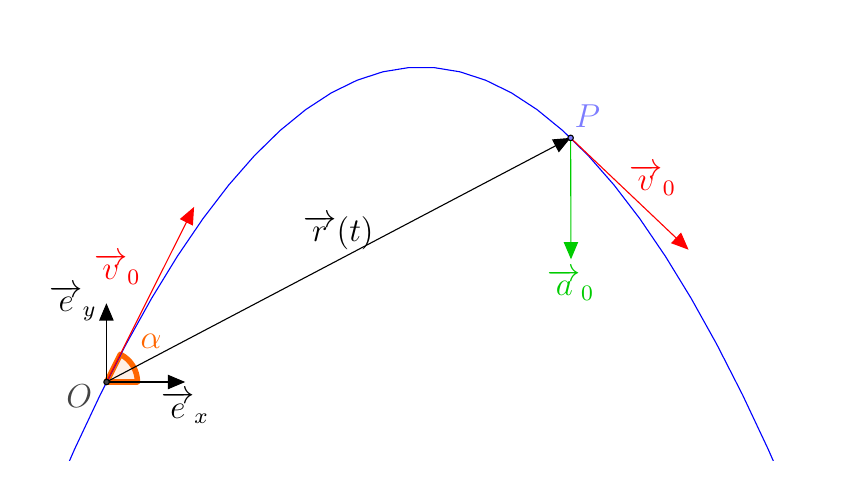
\begin{tikzpicture}[line cap=round,line join=round,>=triangle 45,x=1.0cm,y=1.0cm]
\clip(-1.,-1.) rectangle (9.,4.5);
\draw [shift={(0.0018079900265860363,0.)},line width=2.pt,color=ffwwqq,fill=ffwwqq,fill opacity=0.10000000149011612] (0,0) -- (0.:0.3925823152630728) arc (0.:63.44116603320462:0.3925823152630728) -- cycle;
\draw [samples=50,rotate around={-180.:(4.,3.9992768628452935)},xshift=4.cm,yshift=3.9992768628452935cm,line width=0.4pt,color=qqqqff,domain=-7.994214902762348:7.994214902762348)] plot (\x,{(\x)^2/2/1.998553725690587});
\draw [->,line width=0.4pt,color=ffqqqq] (0,0) -- (1.1133634707356288,2.2237141711451285) node [midway, anchor=south east]{$\vec v_0$};
\draw [->,line width=0.4pt] (0,0.) -- (0.,1.)node [anchor=east]{$\vec e_y$};
\draw [->,line width=0.4pt] (0,0.) -- (1.,0.) node [anchor=north]{$\vec e_x$};
\draw [->,line width=0.4pt] (0,0.) -- (5.895537446451206,3.1003612708570922) node [midway, anchor= south] {$\vec r (t)$};
\draw [->,line width=0.4pt,color=qqccqq] (5.895537446451206,3.1003612708570922) -- (5.9,1.55854) node [anchor=north]{$\vec a_0$};
\draw [->,line width=0.4pt,color=ffqqqq] (5.895537446451206,3.1003612708570922) -- (7.393075087098776,1.6800148279128146);
\draw [fill=uuuuuu] (0.0018079900265860363,0.) circle (1.0pt);
\draw[color=uuuuuu] (-0.3436358197316432,-0.17536988066984197) node {$O$};
\draw [fill=xdxdff] (5.895537446451206,3.1003612708570922) circle (1.0pt);
\draw[color=xdxdff] (6.107800227758184,3.3709570338732475) node {$P$};
\draw[color=ffqqqq] (6.9387661283983535,2.5661632875839486) node {$\vec v_0$};
\draw[color=ffwwqq] (0.568680740180397,0.51721243459322928) node {$\alpha$};
\end{tikzpicture}
}
\end{minipage}
\begin{minipage}{.49\linewidth}
\setlength{\parskip}{.3em}
\begin{equation}
\label{eq:2.29}
\vec a (t) = \vec g + \vec{cste}
\end{equation}

\begin{equation}
\label{eq:2.30}
\vec v (t) = \vec g \cdot t + \vec{v_{0}}
\end{equation}

\begin{equation}
\label{eq:2.31}
\vec r (t) = \frac{1}{2}\vec g \cdot t^{2} + \vec{v_{0}} \cdot t
\end{equation}
où $$\vec g = -g \cdot \vec{e_{y}}$$ et $$\vec{v_{0}} =
\underbrace{V_{0} \cdot \cos(\alpha)}_{v_{0_{x}}} \cdot \vec{e_{x}} +
\underbrace{v_{0} \cdot \sin(\alpha)}_{v_{0_{y}}} \cdot \vec{e_{y}}$$ 
\end{minipage}
\end{center}


\begin{itemize}
\item Hauteur maximale $h: \vec{v_{y}} (t_{h}) = 0$ 

\begin{equation}
\label{eq:2.32} 
\vec{V_{y}} (t_{h}) \stackbin{\eqref{eq:2.30}}{=} - y \cdot t_{h}
+ \vec{v_{0_{y}}} = 0 \implies t_{h} = \frac{\vec{v_{0_{y}}}}{y} =
\frac{\vec{v_{0}} \cdot \sin(\alpha)}{y}
\end{equation}

\begin{equation}
\label{eq:2.33}
h = y (t_{h}) \stackbin{\eqref{eq:2.31}}{=} -\frac{1}{2} \cdot g
\cdot t_{h}^{2} + \vec{v_{0_{y}}} \cdot t_{h}
\stackbin{\eqref{eq:2.32}}{=} \frac{\vec{v_{0}}^{2} \cdot \sin^{2}(\alpha)}{2g}
\end{equation}

\pagebreak

\item Temps de vol: $y (t_{v}) = 0$ 

$$ y (t_{h}) \stackbin{\eqref{eq:2.31}}{=} -\frac{1}{2} \cdot g \cdot
t_{h}^{2} + \vec{v_{0_{y}}} \cdot t_{h} = 0 \implies t_{v} \cdot
\left(-\frac{1}{2} \cdot g \cdot t_{v} + \vec{v_{0_{y}}}\right) $$

\begin{equation}
\label{eq:2.34}
\implies t_{v} = 0 \quad \text{ ou }\quad  t_{v} = \frac{2 \cdot \vec{v_{0_{y}}}}{g}
= \frac{2 \cdot \vec{v_{0}} \cdot \sin(\alpha)}{g}
\end{equation}


\markDate{7/03/2019}

\item Distance horizontale (portée): 
\begin{equation}
\label{eq:2.35}
d = x (t_{v}) \stackbin{\eqref{eq:2.31}}{=} v_{0_{x}} \cdot
t_{v} = \frac{2 \cdot v_{0}^{2} \cdot \cos(x) \cdot \sin (x)}{g}
= \frac{v_{0}^{2} \cdot \sin (2\alpha)}{g}
\end{equation}

\item Équation de la trajectoire $\Gamma$:

\begin{equation}
\label{eq:2.36}
\eqref{eq:2.28}: g (x) = -\frac{a_{0}}{2 v_{0_{x}}^{2}} \cdot
x^{2} + \frac{v_{0_{y}}}{v_{0_{x}}} \cdot x = - \frac{g}{2 v_{0}
\cdot \cos^{2}(\alpha)}
\end{equation}

\item Point de la trajectoire $P (x_{p}, y_{p})$: (où $\frac{1}{\cos^{2}(\alpha)}
= 1 + \tan^{2}(\alpha)$)

$$ \eqref{eq:2.36}: y_{p} = -\frac{g}{2 v_{0}^{2}} \cdot (1 + \tan^{2}(\alpha))
\cdot x_{p}^{2} + \tan(\alpha) \cdot x_{p}$$

\begin{equation}
\label{eq:2.37}
\implies \frac{g \cdot x_{p}^{2}}{2 v_{0}^{2}} \cdot \tan^{2}(\alpha)
- x_{p} \cdot (1 + \tan(\alpha)) + \frac{g \cdot x_{p}^{2}}{2
v_{0}^{2}} + y_{p} = 0
\end{equation}

C'est une équation du $2^\circ$ degrés en $\tan(x)$ qui est fonction
de la vitesse initiale $\vec{v_{0}}$ et des coordonnées $x_{p}$ et $y_{p}$ du
point $P$.

\item Discriminent de l'équation du $2^{\circ}$ ordre en $\tan(\alpha) \eqref{eq:2.37}$ 

\begin{equation}
\Delta  = x_{p}^{2} - 4 \cdot \frac{g \cdot x_{p}^{2}}{2 v_{0}^{2}}
\cdot \left( \frac{g \cdot x_{p}^{2}}{2 v_{0}^{2}} + y_{p}\right)
= x_{p}^{2} \cdot \left( 1 - \frac{2g}{v_{0}^{2}} \cdot \left(
\frac{g x_{p}^{2}}{2 v_{0}^{2}} + y_{p}\right)\right)
\end{equation}

\item On doit distinguer 3 cas:

\begin{enumerate}
\item $\Delta > 0$: il y a deux angles $\alpha$ possibles (angles
complémentaire). Le point $P$ est à portée du canon avec deux
trajectoire possibles.

\item $\Delta = 0$  il y a un angle $\alpha$ possible. Tous les
points $(x, y)$ vérifiant $\Delta = 0$ se trouvent une
parabole, dite de sécurité, d'équation.

\begin{equation}
\label{eq:2.39}
y (x) = - \frac{g}{2v_{0}^{2}} \cdot x^{2} + \frac{v_{0}^{2}}{2g}
\end{equation}

\item $\Delta < 0:$ il n'y a donc pas d'angles de tir possible. $P$
est au delà de la parabole de sécurité.
\end{enumerate}
\end{itemize}


\end{document}
